% !TEX encoding = UTF-8 Unicode
\documentclass[fr]{../../../eplsummary}
\usepackage{framed}

\makeatletter
\renewcommand*\env@matrix[1][*\c@MaxMatrixCols c]{%
  \hskip -\arraycolsep
  \let\@ifnextchar\new@ifnextchar
  \array{#1}}
\makeatother

\hypertitle[']{Algèbre}{1}{EPL}{1101}{Philippe Dan}{Raphaël Jungers et Vincent Wertz}

%Beginning
\newpage

\tableofcontents

\section{Calcul matriciel}
\subsection{Equation matricielle}
Une équation matricielle se traduit par la forme :
\begin{equation}
    Ax = B
\end{equation}
\subsection{Définition d'une matrice}
Une matrice $m\times n$ est un tableau rectangulaire de $m$ lignes et $n$ colonnes. Si $m=n$, alors la matrice est carrée. Toutes les entrées d'une même matrice sont du même type.
\subsection{Addition de matrices}
L'addition de matrices n'est possible que pour des matrices de même genre. L'addition se fait alors en additionnant un élément de la première matrice avec son élément homologue. Le résultat donne alors lieu à une matrice de même genre que les matrices initiales.
\subsection{Multiplication de matrices}
La multiplication de matrice n'est possible que lorsque la première matrice a autant de colonnes que la deuxième matrice a de lignes.
\begin{equation}
    A^{m\times n} \times B^{n\times p} = C^{m\times p}
\end{equation}
Il existe plusieurs manières pour calculer la matrice C.
\subsubsection{Dot product (ligne par colonne)}
\begin{equation}
    C_{i,j} = A_{i,*} \cdot B_{*,j}
\end{equation}
\subsubsection{Colonne par colonne}
\begin{equation}
    \begin{bmatrix}
    3&2&1 \\
    0&4&5\\
    2&7&1
    \end{bmatrix}
    \times
    \begin{bmatrix}
    a\\b\\c
    \end{bmatrix}
    =
    \begin{bmatrix}
    3a+2b+c\\
    0a+4b+5c\\
    2a+7b-c
    \end{bmatrix}
    =
    \begin{bmatrix}
    3\\0\\2
    \end{bmatrix} a +
    \begin{bmatrix}
    2\\4\\7
    \end{bmatrix} b +
    \begin{bmatrix}
    1\\5\\-1
    \end{bmatrix} c
\end{equation}
On remarque ainsi que chaque colonne de AB est une combili des colonnes de A.
\subsubsection{Ligne par ligne}
\begin{gather}
    \begin{bmatrix}[cc]
    1&2\\3&4
    \end{bmatrix}
    \begin{bmatrix}[ccc]
    1&2&3\\4&5&6
    \end{bmatrix} =
    \begin{bmatrix}[cc]
        \begin{pmatrix}[cc]
        1&2
        \end{pmatrix}
        \begin{pmatrix}[ccc]
        1&2&3 \\ 4&5&6
        \end{pmatrix} \\
        \begin{pmatrix}[cc]
        3&4
        \end{pmatrix} &
        \begin{pmatrix}[ccc]
        1&2&3 \\ 4&5&6
        \end{pmatrix}
    \end{bmatrix}
\end{gather}
Chaque ligne de AB est donc une combili des lignes de B.
\subsubsection{Colonne par ligne}
\begin{equation}
    \begin{bmatrix}
    3&2&1 \\
    0&4&5\\
    2&7&1
    \end{bmatrix} 
    \begin{bmatrix}
    a&d\\
    b&e\\
    c&f
    \end{bmatrix} =
    \begin{bmatrix}
    3a+2b+c&3d+2e+f \\
    4b+5c&4e+5f\\
    2a+7b-c&2d+7e-f
    \end{bmatrix} =
    \begin{bmatrix}
    3\\0\\2  
    \end{bmatrix}
    \begin{bmatrix}
    a&d
    \end{bmatrix}+
    \begin{bmatrix}
    2\\4\\7
    \end{bmatrix}
    \begin{bmatrix}
    b&e
    \end{bmatrix}+
    \begin{bmatrix}
    1\\5\\-1
    \end{bmatrix}
    \begin{bmatrix}
    c&f
    \end{bmatrix}
\end{equation}
\subsection{Matrice identité}
La matrice identité est carrée et a comme spécificité que tous les éléments de sa diagonale valent 1, les autres étant nuls.
\begin{equation}
    \mathbb{1} = 
    \begin{bmatrix}
    1&0 \\
    0&1
    \end{bmatrix}
\end{equation}
\subsubsection{Particularités}
    Si $A_{m\times n}$ avec $ m \leq n$, alors il existe peut-être $B_{n\times n}$ tel que : $AB = \mathbb{1}$ $B$ est alors inverse à droite de A et n'est pas unique.
    \\ \indent Si $A_{n\times n}$ alors $B$ existe peut-être et est unique.
\subsection{Opération par blocs}
Soient $A,B,C,D,E,F,G,H$ des matrices, alors on a :
\begin{equation}
    \begin{bmatrix}
    A&B\\
    C&D
    \end{bmatrix}
    \begin{bmatrix}
    E&F\\
    G&H
    \end{bmatrix} =
    \begin{bmatrix}
    AE+BG&AF+BH\\
    CE+DG&CF+DH
    \end{bmatrix}
\end{equation}
Pour autant que les dimensions des matrices soient compatibles.
\subsection{Matrices Inversibles}
Soit $A_{n\times n}$, A est inversible ssi :
\begin{equation}
    \exists B : AB = BA = \mathbb{1} \Rightarrow B = A^{-1}
\end{equation}
\subsubsection{Propriétés}
L'inverse est unique. C'est-à-dire que :
\begin{equation}
    A\Vec{x} = \Vec{b} \Rightarrow \Vec{x} = A^{-1}\Vec{b} \quad \text{solution unique}
\end{equation}
Si $\Vec{x}\ne 0$ et $A\Vec{x} = 0$, alors A n'est pas inversible. Autrement dit, s'il est possible de trouver une combili non nulle de $A$ qui donne la matrice nulle, alors $A$ n'est pas inversible car il est impossible de revenir de la matrice nulle vers la matrice initiale $\Vec{x}$. 
\subsection{Calcul de l'inverse}
\begin{gather}
    (AB)^{-1} = B^{-1}A^{-1} \quad \text{car} \\
    (AB)\cdot (AB)^{-1} = AB\cdot B^{-1}A^{-1} = A\cdot \mathbb{1} \cdot A^{-1} = \mathbb{1}
\end{gather}
\subsubsection{Méthode de Gauss-Jordan}
On part de la matrice étendue $A:\mathbb{1}$ et on lui fait subir une série d'opérations linéaires jusqu'à ce qu'on ait à gauche la matrice identité. Il reste alors à droite la matrice inverse de $A$.
\begin{equation}
    \begin{bmatrix}[cc|cc]
        a&b&1&0 \\
        c&d&0&1
    \end{bmatrix}
\end{equation}
\subsubsection{Propriétés}
Si $A$ est diagonale (carrée), $A$ est inversible ssi aucun élément diagonal n'est nul.
\newline \indent Si $A$ est diagonalement dominante, alors A est inversible.
\begin{equation}
    |a_{i,i}| > \sum_{j\ne i}|a_{i,j}|
\end{equation}
\subsection{Matrice transposée}
On appelle matrice transposée $A^T$ de $A$ la matrice telle que les lignes de A sont les colonnes de $A^T$ et les colonnes de $A$ sont les lignes de $A^T$.
\subsubsection{Propriétés}
\begin{gather}
    (A^T)^T = A \\
    (A + B)^T = A^T + B^T \\
    (AB)^T = B^TA^T \\
    (A^{-1})^T = (A^T)^{-1} 
\end{gather}
\subsubsection{Matrice symétrique}
Une matrice est symétrique lorsqu'elle est carrée et lorsque $A=A^T$. Si son inverse existe, alors elle est également symétrique.
\subsection{Résolution de systèmes d'équations}
Si l'on considère un système d'équations linéaires de $m$ équations à $n$ inconnues, alors ce système peut se traduire par :
\begin{gather}
    A_{m\times n} \cdot X_{n\times 1} = B_{m\times 1}
\end{gather}
On a alors deux interprétations possibles :
\begin{itemize}
    \item Via le dot product, on retrouve chacune des équations
    \item Si l'on considère le produit $A_{*1}.x_1 + A_{*2}.x_2 + ... + A_{*n}.x_2 = B$, alors on peut l'interpréter comme : "Est-ce que b est une combinaison linéaire des colonnes de A ?".
\end{itemize}
Pour résoudre un tel système on peut utiliser la méthode de l'échelonnement, c'est-à dire soustraire un multiple bien choisi de l'équation une pour avoir des "zéros" dans les autres équations, tout en répétant l'opération jusqu'à avoir une matrice échelonnée, c'est-à-dire où le premier élément non nul d'une ligne est précédé par n zéros où n est un nombre supérieur au nombre de zéros de la ligne précédente. Il faut ainsi que l'élément 1,1 soit différent de 0.
\subsubsection{Cas de figures}
\begin{enumerate}
    \item Si on a $(0\, 0\, X_1 = x)$ alors le système est possible et on a une solution unique obtenue par substitution classique.
    \item Si on a $(0\, 0\, 0 = 0)$, le système est indéterminé et il y a une infinité de solutions.
    \item Si on a $(0\, 0\, 0 = x)$, le système est impossible.
    \item Si on a $(0\, 0\, X_1\, X_2 = x)$, le système est également indéterminé et il y a une infinité de solutions.
\end{enumerate}
\begin{framed}
De façon générale, si $n > m$, alors le système admet soit une infinité de solutions, soit aucune solution.
\end{framed}
\subsection{Échelonnement de Gauss-Jordan}
On peut échelonner une matrice de telle sorte à ce que chaque élément au-dessus des pivots soit égal à 0 et que chaque pivot soit égal à 1. On l'appelle la matrice échelonnée réduite. Cette matrice est unique.
\begin{gather}
    R = \begin{bmatrix}[cccc]
    1&0&X&0 \\
    0&1&0&0 \\
    0&0&0&1 \\
    \end{bmatrix}
\end{gather}
\begin{framed}
Si A est carrée, alors sa forme de G-J, soit possède \emph{au moins} une ligne de zéros, soit vaut la matrice identité.
\end{framed}
\subsection{Matrices élémentaires}
Lorsque l'on effectue des opérations sur les lignes d'une matrice A (sur les colonnes à éviter car on change les variables), on peut résumer ces opérations par des matrices qui pré-multiplient la matrice A. On les appelle les matrices élémentaires. Par exemple :
\begin{gather}
    L_2 \leftarrow L_2 - L_1 \Rightarrow 
    \begin{bmatrix}[ccc]
    1&0&0 \\ -1 & 1 & 0 \\ 0&0&1
    \end{bmatrix}
\end{gather}
\begin{framed}
Les matrices élémentaires sont inversibles.
\end{framed}
\subsubsection{Factorisation LU}
Soit A, une matrice carrée sans besoin de permuter les lignes. Si on prend la forme échelonnée de A, on aura ainsi une matrice $U$ triangulaire supérieure. Ainsi, l'ensemble des matrices inverses des matrices élémentaires nécessaires pour échelonner la matrice $A$, forment une matrice $L$ triangulaire inférieure.
\begin{gather}
    A = \underbrace{E_{1}^{-1}E_{2}^{-1}E_{3}^{-1}...E_{n}^{-1}}_{L}\cdot\, U
\end{gather}
\paragraph{Résolution de systèmes grâce à la méthode LU}
Cette méthode s'avère très efficace dans la résolution de systèmes car elle permet de décomposer la résolution et ainsi résoudre :
$\begin{cases}
    Ux = C \\
    LC = b
\end{cases}$
Si on veut $U$ avec 1 sur ses pivots, alors on a $A = LDU$, pourvu que A soit inversible.
\subsection{Déterminant d'une matrice}
Soit la matrice carrée A. On a ces propriétés qui s'appliquent :
\begin{itemize}
    \item Si det A = 0, la matrice n'est pas inversible
    \item Det $A^{-1}$ = $\frac{1}{det A}$
    \item det $\mathbb{1}$ = 1
    \item det est unique
    \item Pour chaque permutation de lignes (ou colonnes) le déterminant change de signe
    \item $det\left(\begin{bmatrix}[cc]ta & tb \\c & d \end{bmatrix}\right) $ = $t\cdot det\left(\begin{bmatrix}[cc]a & b \\c & d \end{bmatrix}\right) $
    \item $det\left(\begin{bmatrix}[cc]a+a' & b+b' \\c & d \end{bmatrix}\right) $ = $det\left(\begin{bmatrix}[cc]a & b \\c & d \end{bmatrix}\right) $ + $det\left(\begin{bmatrix}[cc]a' & b' \\c & d \end{bmatrix}\right) $
    \item Si deux lignes sont multiples l'une de l'autre, alors le déterminant vaut 0
    \item Si la matrice possède une ligne ou une colonne de 0, alors le déterminant vaut 0
    \item det $A^T$ = det A
    \item Si A est triangulaire, alors $det A =$ produit des termes sur la diagonale
    \item $det(AB) = det(A) \cdot det(B)$
\end{itemize}
Pour une matrice $2\times 2$, le déterminant vaut : $ab-cd$. Pour trouver rapidement le déterminant d'une matrice, on peut recourir à la méthode U.
\begin{itemize}
    \item Si $E_m : L_i \leftarrow L_j$ alors $det(E_m) = -1$
    \item Si $E_n : L_i \leftarrow L_i + \lambda L_j$ alors $det(E_n) = 1$
    \item Si $E_k : L_i \leftarrow \alpha L_j$ alors $det(E_k) = \alpha $
\end{itemize}
Ainsi par exemple, si on prend :
\begin{gather}
    \begin{bmatrix}[ccc]
    0 & 1 & -1 \\
    2 & 1 & 3 \\
    1 & 0 & 4
    \end{bmatrix}
    \xRightarrow{det \,-1}
    \begin{bmatrix}[ccc]
    1 & 0 & 4 \\
    2 & 1 & 3 \\
    0 & 1 & -1
    \end{bmatrix}
    \xRightarrow{det \,-1}
    \begin{bmatrix}[ccc]
    1 & 0 & 4 \\
    0 & 1 & -1 \\
    2 & 1 & 3
    \end{bmatrix}
    \xRightarrow{det \,1}
    \begin{bmatrix}[ccc]
    1 & 0 & 4 \\
    0 & 1 & -1 \\
    0 & 1 & -5
    \end{bmatrix}
    \xRightarrow{det \,1}
    \begin{bmatrix}[ccc]
    1 & 0 & 4 \\
    0 & 1 & -1 \\
    0 & 0 & -4
    \end{bmatrix} = U
    \\
    det(U) = -4 \Rightarrow det(A) = (-1)(-1)\cdot det(U) = det(U) = -4
\end{gather}
\section{Espace vectoriel}
\subsection{Définitions et notions}
Un espace vectoriel est un espace de vecteurs n-uples. Ces vecteurs peuvent être composés de Réels, Complexes, Polynômes, fonctions, etc. On considère dans le cours des espaces vectoriels de corps scalaires, donc sur $\mathbb{R}, \mathbb{C}$. Un espace vectoriel doit répondre donc à ces deux critères suivants :
\begin{itemize}
    \item L'addition de vecteurs dans un espace vectoriel donne un vecteur du même type.
    \item La multiplication d'un vecteur par un scalaire résulte un autre vecteur du même type.
\end{itemize}
Ces deux propriétés assurent que toute combili de vecteurs donne un autre vecteur.
\subsection{Propriétés d'un espace vectoriel}
Si l'on considère un espace vectoriel, on a alors $\forall x,y,z \in \mathbb{E}$. On a ces propriétés suivantes qui sont respectées :
\begin{enumerate}
    \item $x + y = y +x$
    \item $x + (y + z) = (x+y)+z$
    \item $\exists 0 : x + 0 = x = 0 +x$
    \item $\exists -x : x + (-x) = 0 = (-x) + x$
    \item $1 \cdot x = x$
    \item $(c_1 c_2 )\cdot x = c_1 (c_2\cdot x)$
    \item $c(x+y)=cx+cy$
    \item $(c_1+c_2)\cdot x = c_1\cdot x + c_2 \cdot x$
\end{enumerate}
\subsection{Sous-espace vectoriel}
Un sous-espace vectoriel est un sous-ensemble d'un espace vectoriel, lui-même espace vectoriel. Ce sous-espace vectoriel est valable si et seulement si $\forall x,y \in \mathbb{V} \in \mathbb{E} : \quad x + y \in \mathbb{V}$ et $c\cdot x \in \mathbb{V}$, autrement dit, si  $\forall x,y \in \mathbb{v} : \quad \alpha x + \beta y \in \mathbb{V}$.
\subsubsection{Propriétés}
L'intersection de plusieurs sous-espaces vectoriels donne un sous-espace vectoriel. L'addition de plusieurs sous-espaces vectoriels donne un sous-espace vectoriel.
\paragraph{Somme directe}
La somme est dite directe si lorsque l'on fait la somme, l'intersection des vecteurs donne le vecteur nul. Autrement dit, la dimension de l'espace généré par l'intersection des différents espaces est l'espace nul.
\subsection{Sous-espace vectoriel engendré}
Le sous-espace vectoriel engendré est défini comme l'ensemble de toutes les combinaisons linéaires de $v_1,v_2,...,v_n$.
\subsubsection{Espace colonne}
On note $C(A)$ le sous-espace vectoriel engendré par les colonnes de $A^{m\times n}$. Si $b \in C(A)$, alors le système possède au moins une solution. $C(A) \subset R^m$.
\subsubsection{Espace annulateur de A}
On note $N(A)$ le sous-espace vectoriel engendré par les solutions de $Ax = 0$. $N(A) \subset R^n$.
\subsection{Forme échelonnée réduite}
Si l'on échelonne la matrice $A$ de sorte à ce que les pivots valent 1 et que les éléments au-dessus des pivots soient nuls, alors on a la forme échelonnée réduite de la matrice $A$. Les colonnes qui possèdent un pivot déterminent des variables pivots, là où les colonnes sans pivots déterminent des variables libres.
\subsubsection{Résolution de $Ax = 0$}
On prend la forme échelonnée réduite de $A$ et l'on établit des solutions spéciales à partir des variables libres. Ces solutions spéciales forment les bases de l'espace annulateur.
\subsubsection{Rang d'une matrice}
On définit le rang d'une matrice par rapport à son nombre de pivots.
\subsection{Solutions complètes de $Ax = b$}
On a $[A:b] \rightarrow [R:d]$. Si d possède des composantes non nulles pour les lignes nulles de R, alors il n'y a pas de solution.
\newline \indent Sinon, il faut chercher une solution particulière $Ax_p = b$ en posant par exemple les variables libres à 0 et on obtient les variables pivots par correspondance.
\begin{framed}
L'ensemble des solutions est alors déterminé par :
\begin{equation}
    x = x_p + c_1\cdot v_1 + ... +C_{n-r}\cdot v_{n-r}
\end{equation}
où $v_n$ sont les solutions de $Ax = 0$. Il est possible de démontrer que ces solutions sont les seules possibles pour le système $Ax = b$. Pour ce faire, il faut poser $Y_1, Y_2$ solutions du système et faire leur différence.
\end{framed}
\subsubsection{Cas particuliers}
\paragraph{Premier cas}
\begin{itemize}
    \item Si chaque colonne de $A$ donne un pivot, la forme échelonnée réduite est alors : $\begin{bmatrix}[c] I \\ 0 \end{bmatrix}$. 
    \item Il n'y a alors pas de variables libres, A est de plein-rang : $r = n \Rightarrow m \geq n$. 
    \item $N(A) = {0}$
    \item $Ax = b$ possède au plus une solution.
\end{itemize}
\paragraph{Second cas}
\begin{itemize}
    \item Si chaque ligne de $A$ donne un pivot, la forme échelonnée réduite ne possède pas de lignes nulles.
    \item A est de plein-rang : $r = m \Rightarrow n \geq m$. 
    \item $N(A)$ est engendré par $n-r = n-m$ vecteurs. Il y a donc $n-m$ variables libres
    \item $Ax = b$ possède au moins une solution.
\end{itemize}
\subsection{Indépendance linéaire}
Les colonnes d'une matrice $A$ sont indépendantes si $Ax=0$ admet seulement la solution $x = 0$.
\subsubsection{Suite libre}
On appelle ainsi suite libre, une suite de vecteurs dont la seule combili de ces vecteurs donnant le vecteur nul est la combinaison nulle.
\begin{gather}
    0v_1 + 0v_2+...+0v_n = 0
\end{gather}
Par convention, une suite vide est libre.
\subsubsection{Suite génératrice}
Toute suite de vecteurs donnant place à un espace dont chaque vecteur est une combili de la suite proprement-dite est appelée suite génératrice.
\begin{itemize}
    \item L'espace colonne $C(A)$ est engendré par les colonnes de A
    \item L'espace ligne de A est engendré par les colonnes de $A^T$
    \item L'espace annulateur de A est engendré par les $n-r$ solutions spéciales de $Ax = 0$
\end{itemize}
Par convention, une suite vide engendre l'espace ${0}$
\subsection{Bases d'un sous-espace}
Une base d'un sous-espace vectoriel est une suite libre et génératrice de cet espace vectoriel.
\subsubsection{Dimensions}
\begin{itemize}
    \item Tout espace vectoriel engendré par un nombre fini de vecteurs admet une base.
    \item Si $(e_1,...,e_n)$ est une base de E, alors tout vecteur de E s'écrit comme une combili unique des vecteurs de cette suite.
\end{itemize}
\begin{framed}
Toutes les bases d'un même espace vectoriel ont le même nombre d'éléments. Ce nombre est la \emph{dimension} de l'espace vectoriel.
\end{framed}
\subsection{Les quatres sev liés à une matrice}
\begin{itemize}
    \item L'espace colonne $C(A)$ de dimension : $r$
    \item L'espace annulateur $N(A)$ de dimension : $n-r$
    \item L'espace ligne $C(A^T)$ de dimension : $r$
    \item L'espace annulateur $N(A^T)$ de dimension $m-r$
\end{itemize}

\section{Les applications linéaires}
\subsection{Définitions}
Considérons $E et F$ deux espaces vectoriels. On a alors que l'application $A : E \rightarrow F$ est linéaire si :
\begin{gather}
    A(x\alpha + y\beta) = \alpha A(x) + \beta A(y)
\end{gather}
pour tout $x,y \in E$ et $\alpha ,\beta \in K$ où $K$ désigne un corps de scalaire.
\newline \indent De manière générale, on a donc : 
\begin{gather}
    A(\Sigma x_i \alpha_i) = \Sigma \alpha_i A(x_i)
\end{gather}
\subsubsection{Kernel et Range}
Comme pour les espaces vectoriels, on définit pour une application linéaire les notions suivantes : 
\begin{itemize}
    \item $Im(L) = \left\{ L(x) \left| \right. x \in V \right\}$ l'image de L
    \item $Ker(L) = \left\{ x : L(x) = 0 \left| \right. x \in V \right\}$ le noyau de L
\end{itemize}
On a donc pour toute application linéaire que l'image de $L : V\rightarrow W$ est un sous-espace vectoriel de W et le noyau de L est un sous-espace vectoriel de V.
\paragraph{Surjectivité et injectivité}
Une application linéaire est dite surjective si $Im(L) = W$, autrement dit si tout l'espace d'arrivée est rempli par le sous-espace vectoriel image de L.
\newline \indent Une application linéaire est dite injective si $L(X) = L(Y) \Rightarrow x = y$, autrement dit si chaque élément de $Im(L)$ est l'image d'un seul et unique point.
\subsubsection{Inversibilité}
Soit A une application linéaire $A : E \rightarrow F$
\begin{itemize}
    \item A est inversible à droite si $\exists K : AK = \mathbb{1}_F$
    \item A est inversible à gauche si $\exists K : KA = \mathbb{1}_E$
    \item A est inversible si elle est inversible à gauche et à droite.
\end{itemize}
\subsubsection{Lien entre application et matrice}
Une application linéaire peut se traduire par une matrice $A$ dont les colonnes sont les images des vecteurs de la base canonique de l'application linéaire.
\paragraph{Injectivité et surjectivité}
\begin{itemize}
    \item L'application linéaire est injective ssi $N(A) = 0$
    \item Elle est surjective ssi $C(A) = F$
\end{itemize}
\subsubsection{Solution d'un système}
Considérons $A : E\rightarrow F$ et $b \in F$. Prenons une solution particulière $u \in E : Au = b$. 
\begin{framed}
Alors l'ensemble des solutions de $Ax = b$ sont : $u + Ker(A) = \{u + v | v \in Ker(A)\}$
\end{framed}
\subsubsection{Dimensions}
Soit $A : E \rightarrow F$. On a :
\begin{framed}
    $dim(E) = dim(Ker(A)) + dim(Im(A))$
\end{framed}
\subsubsection{Liens importants}
Soit $A : E \rightarrow F$. On a $dim(E) = n$ et $dim(F) = m$. On a alors les relations suivantes 1,2,3 qui sont équivalentes, de même pour 1',2',3'.
\newline \newline
\begin{minipage}{\linewidth}
    \begin{minipage}{.45\linewidth}
    \begin{enumerate}
        \item A est injective
        \item Dim (Ker(A)) = 0
        \item Rang de A = n
    \end{enumerate}
    \end{minipage}
    \begin{minipage}{.45\linewidth}
    \begin{enumerate}
        \item[1'] A est surjective
        \item[2'] Dim (Ker(A)) = n-m
        \item[3'] Rang de A = m
    \end{enumerate}
    \end{minipage}
\end{minipage}
Si les deux conditions sont réunies,$n=m$, alors A est bijective.
\paragraph{Inversibilité et bijection}
\begin{minipage}{\linewidth}
    \begin{minipage}{.45\linewidth}
        \begin{framed}
            Si A est injective, alors elle est inversible à gauche.
        \end{framed}
    \end{minipage}
    \begin{minipage}{.45\linewidth}
        \begin{framed}
            Si A est surjective, alors elle est inversible à droite.
        \end{framed}
    \end{minipage}
\end{minipage}
\paragraph{Preuve de l'inversibilité à droite}
Soit $A \in \mathbb{R}^{m\times n}$. A est surjective ssi elle est inversible à droite.
\paragraph{1}
Supposons que A est surjective, par définition on a : $\forall y \in \mathbb{R}^m,\exists X \in \mathbb{R}^n : Ax = y$.
\begin{gather}
    \text{Donc, pour } \quad y_1 = \begin{bmatrix}[c]1\\0\\\vdots \\0\end{bmatrix} \quad y_2 = \begin{bmatrix}[c]0\\1\\\vdots \\0\end{bmatrix} \quad y_n = \begin{bmatrix}[c]0\\0\\\vdots \\n\end{bmatrix} \quad \text{On obtient respectivement} \\
    x_i : Ax_i = y_i \quad \text{on obtient donc} A[x_1,x_2,\dots,x_n] = \begin{bmatrix}[ccccc]
    1&&&&\\
    &1&&&\\
    &&1&&\\
    &&&\ddots&\\
    &&&&1
    \end{bmatrix}
\end{gather}
\paragraph{2}
Supposons que A est inversible à droite. Soit $y \in \mathbb{R}^m$.
\begin{gather}
    \exists B \in \mathbb{R}^{n\times m} : AB = \mathbb{1}_m \\
    ABy = y \\
    \text{En posant} \quad x = By \quad \text{on obtient la thèse}
\end{gather}
\subsection{Changement de base}
Soit $A: E \rightarrow F$. Prenons deux bases V,W de E,F. Alors dans les bases V,W, la matrice A s'exprime :
\begin{equation}
    _WA_V := W^{-1}AV
\end{equation}
\subsection{Déterminant d'une matrice}
Le déterminant d'une matrice est bien défini et ne varie pas en fonction des opérations linéaires sur la matrice.
\section{Espaces euclidiens}
\subsection{La notion de norme, distance}
La notion de distance dans un espace vectoriel peut être définie sous le nom de norme. Cette norme peut être définie sous différents aspects, mais elle doit impérativement posséder ces propriétés :
\begin{itemize}
    \item La norme est positive ou nulle (si à l'origine)
    \item Elle est sous additive : $||x+y||\leq ||x|| + ||y||$
    \item Elle est homogène : $||\alpha\cdot x|| = ||\alpha||\cdot ||x||$
\end{itemize}
\subsubsection{Norme euclidienne}
La norme euclidienne est définie comme suit :
\begin{gather}
    ||x|| = \sqrt{x^Tx}
\end{gather}
\subsection{L'espace euclidien}
Pour que cette notion de norme euclidienne fonctionne, il faut que l'espace soit euclidien, c'est-à-dire un espace vectoriel muni du produit scalaire. C'est-à-dire une fonction :
\begin{itemize}
    \item Bilinéaire :
    \begin{itemize}
        \item $(\alpha x + \beta y | z) = \alpha (x|z) + \beta (y|z)$
    \end{itemize}
    \item Symétrique : $(x|z) = (z|x)$
    \item Défini positif partout : $(x|z) \geq 0$
\end{itemize}
\subsubsection{Propriétés du produit scalaire}
\begin{itemize}
    \item $||x|| \geq 0$ et $dist(x,y) \geq 0$
    \item $||\alpha x|| = \alpha ||x||$
    \item Inégalité de Cauchy-Schwartz : $(x|z) \leq ||x||\cdot ||z||$
    \item Inégalité triangulaire : $||x+y|| \leq ||x|| + ||y||$
\end{itemize}
\subsection{Orthogonalité}
Deux vecteurs sont orthogonaux si $(x|z) = 0$. On appelle espace orthogonal d'un espace vectoriel V, sous espace de E : ${x \in E| (x|v)=0 \forall v \in V}$
\subsubsection{Propriétés}
\begin{itemize}
    \item $V^\perp$ est un sev de E
    \item Seul x = 0 appartient à $V^\perp \cap V$
    \item $E^\perp = 0$ et inversement
    \item Si $V_1 \subseteq V_2$ alors, $V_2^\perp \subseteq V_1^\perp$
    \item Si $V_1,V_2$ sont deux sev, alors $(V_1+V_2)^\perp = V_1^\perp \cap V_2^\perp$
    \item $(C(A^T)) \perp N(A)$ et $C(A) \perp N(A^T)$
\end{itemize}
L'espace ligne et l'espace annulateur sont complémentaires donc, de même pour l'espace colonne et l'espace annulateur de la transposée !
\subsubsection{Projection orthogonale}
Soit E un espace euclidien et V un sous-espace de E. On a que la projection orthogonale de E sur V est une application linéaire telle que $x - P_v(x) \in V^\perp $. En outre, la projection orthogonale est bien définie, elle est unique.
\subsubsection{Projection sur une ligne}
La projection d'un vecteur b sur la droite passant par a est le point p tel que :
\begin{gather}
    p = a(\frac{a^Tb}{a^Ta}) = a\hat{x} \\
    \text{Pour obtenir la matrice de projection générale, on prend :} \\
    P = \frac{aa^T}{a^Ta} \Rightarrow p = P\cdot b
\end{gather}
\paragraph{Projection sur un sous-espace}
Il faut trouver une combinaison linéaire telle que $p = A\hat{x}$ est proche de b.
Pour cela, on a :
\begin{gather}
    A^TA\hat{x} = A^Tb \\
    p = A\hat{x} = A(A^TA)^{-1}A^Tb = b \\
    P = A(A^TA)^{-1}A^T
\end{gather}
\paragraph{Propriétés}
\begin{itemize}
    \item $P^T = P$ et $P^2 = P$ et $Pb = p$ \\
    \item Il est possible d'utiliser la méthode des moindres carrés pour approximer un nuage de points par une droite ou une parabole (si 3 points au maximum).
    \item L'erreur obtenue sera minimisée et équilibrée.
\end{itemize}
\paragraph{Erreur de projection}
L'erreur obtenue en projetant est obtenue par :
\begin{gather}
    e = b-p
\end{gather}
L'erreur est perpendiculaire au sous-espace de projection (qui peut être une droite).
\paragraph{Approximation d'une solution}
Si l'on considère une matrice $A : m\times n$ et $b \in \mathbb{R}^m$ où rang $A = n$. Alors, les équations $A^TAx = A^Tb$ ont une solution unique x* qui minimise $|b-Ax|$
\subsubsection{Propriétés}
\begin{itemize}
    \item $P_v$ est une application linéaire
    \item Ker $P_v$ = $V^\perp$
    \item $P_v \circ P_v = P_v$
\end{itemize}
\paragraph{Démonstration de l'unicité de la projection}
\begin{gather}
    \text{Soient} \quad x,y \in V : 
        \begin{cases}
        x-z \in V^\perp \\
        z-y \in V^\perp
        \end{cases}
    \Rightarrow (x-y) \in V \Rightarrow x-y = x-z + z-y \in V^\perp \\
    \text{Donc} \quad (x-y;x-y) = 0 \Rightarrow x-y = 0
\end{gather}
\subsection{Base orthonormée}
Une base de E est orthonormée si tous les vecteurs de la base ont une norme égale à 1 et si les produits scalaires respectifs entre eux valent 0.
\subsubsection{Matrices orthogonales}
Si les colonnes d'une matrice sont orthonormées, alors :
\begin{gather}
    Q^TQ = I
\end{gather}
Si Q est une matrice carrée, alors $Q^T = Q^{-1}$ (Q est orthogonale) \\
La méthode des moindres carrés se résume alors à :
\begin{gather}
    Qx=b \Rightarrow \hat{x} = Q^Tb \\
    P = QQ^T
\end{gather}
\subsubsection{Norme d'un vecteur}
Calculer la norme d'un vecteur dans une base orthonormée revient à calculer :
\begin{gather}
    ||\Vec{x}|| = \sqrt{x^Tx}
\end{gather}
\subsubsection{Expression d'un vecteur}
Dans une base orthonormée, exprimer un vecteur en fonction de la base est très aisée. 
On projette le vecteur sur chaque vecteur de la base et on obtient la composante en fonction de chaque vecteur de la base.
\begin{gather}
    \Vec{v} = (e_1|v)\Vec{e_1} + \cdots + (e_n|v)\Vec{e_n}
\end{gather}
\subsubsection{Produit scalaire}
Dans une base orthonormée, calculer le produit scalaire est aisé. Il suffit de multiplier les différentes composantes entre elles.
\begin{gather}
    (\Vec{x}|\Vec{y}) = x^Ty
\end{gather}
\subsubsection{Base non orthonormée}
Lorsque la base n'est pas orthonormée, il est possible de projeter l'espace vectoriel sur un sous-espace vectoriel orthonormé. Cette méthode s'appelle la procédure de Gram-Schmidt. 
\begin{gather}
    \Vec{q_1} = \frac{\Vec{v_1}}{||\Vec{v_1}||} \\
    \Vec{q_2} = \frac{\Vec{v_2} - (v_2|q_1)\Vec{q_1}}{||\Vec{v_2} - (v_2|q_1)\Vec{q_1}||} \\
    \vdots \\
\end{gather}
Sous forme matricielle, cette méthode donne lieu à une factorisation V = QR. \\
\begin{gather}
    Q = \begin{bmatrix}[ccc]
    q_1&q_2&q_3
    \end{bmatrix}\\
    R = Q^TA =  \begin{bmatrix}[ccc]
    q_1^Ta&q_2^Tb&q_3^Tc\\
    &q_2^Tb&q_3^Tc\\
    &&q_3^Tc
    \end{bmatrix}
    \quad \text{(triangulaire supérieure)}
\end{gather}
La méthode des moindres carrés se résume alors à simplement : 
\begin{gather}
    R^TR\hat{x}=R^TQ^Tb \\
    R\hat{x}=Q^Tb \\
    \hat{x} = R^{-1}Q^Tb
\end{gather}
\begin{framed}
    \begin{itemize}
        \item Toute base orthonormée est une famille libre.
        \item Tout espace vectoriel de dimension finie admet une base orthonormée.
        \item Tout espace vectoriel de dimension finie admet une application linéaire $P_v$ pour la projection orthogonale sur cet espace.
        \item Tout sous-espace V de $\mathbb{R}^n$ est tel que $V \bigoplus V^\perp = \mathbb{R}^n$
        \item C(A) = $N(A^T)^\perp$
        \item N(A) = $C(A^T)^\perp$
    \end{itemize}
\end{framed}
\section{Vecteurs et valeurs propres}
\subsection{Valeurs propres}
Soit une matrice A $n\times n$ et x un vecteur de $\mathbb{R}^n$. On se demande s'il existe des vecteurs particuliers tels que $Ax = \lambda x$.
\begin{itemize}
    \item Le cas x = 0 n'est pas intéressant.
    \item Si le déterminant de A vaut 0 alors, une valeur propre vaut 0.
    \item Si A est la matrice identité, alors une des valeurs propres vaut 1.
    \item De manière générale, pour obtenir les valeurs propres, il faut résoudre :
    \begin{gather}
        det(A-\lambda I) = 0 \quad \text{$A-\lambda I$ est non inversible}
    \end{gather}
\end{itemize}
Chaque valeur propre est une racine (éventuellement complexe) du polynôme caractéristique de $det(A-\lambda I)$.
\begin{gather}
    det(A-\lambda I)=(-1)^n(\lambda-\lambda_1)^{m_1}\cdots(\lambda-\lambda_n)^{m_n} \\
\end{gather}
\subsubsection{Propriétés}
\begin{itemize}
    \item Le produit des valeurs propres = $det(A)$
    \item Les valeurs propres d'une matrice triangulaire sont les éléments sur la diagonale.
    \item La somme des valeurs propres  = $trace(A)$, une valeur bien définie.
    \item A et B ont les mêmes vecteurs propres ssi $AB = BA$
\end{itemize}
\subsection{Vecteurs propres}
Pour trouver les vecteurs propres, il suffit de résoudre le nullspace de $(A-\lambda I) x = 0$ avec chaque valeur propre trouvée. On a donc n vecteurs propres possibles. Tout multiple d'un vecteur propre est également un vecteur propre.
\subsubsection{Approximation de résultats}
On peut approximer le résultat d'une application linéaire exposant un très grand nombre en décomposant le vecteur de base en une combili de vecteurs propres.
\subsection{Diagonalisation}
Supposons que $A \in \mathbb{R}^n$ possède n vecteurs propres. On a :
\begin{gather}
    X = [x_1\,x_2\,x_3\,\cdots x_n] \\
    AX = [\lambda_1x_1 \, \lambda_2x_2 \,\cdots \lambda_nx_n] \\
    AX = [x_1\,x_2\,x_3\,\cdots x_n] \begin{bmatrix}[cccc]
    \lambda_1&0&\cdots&0 \\
    0&\lambda_2&\cdots&0 \\
    &&\ddots& \\
    0&0&\cdots&\lambda_n
    \end{bmatrix} \\
    X^{-1}AX = \Lambda
\end{gather}
\subsubsection{Propriétés}
\begin{itemize}
    \item $A = X\Lambda X^{-1} $\\
    \item $A^k = X\Lambda^k X^{-1}$ \\
    \item $A,\Lambda$ ont les mêmes valeurs propres \\
    \item $A,B = P^{-1}AP$ ont les mêmes valeurs propres \\
    \item A et B sont des matrices semblables \\
    \item Si le polynôme caractéristique de A possède n racines distinctes, alors A est diagonalisable et possède n vecteurs propres indépendants.
\end{itemize}
\subsection{Multiplicité algébrique et géométrique}
La multiplicité algébrique d'une valeurs propres est sa multiplicité comme racine du polynôme caractéristique. La multiplicité géométrique désigne la dimension de l'espace généré par les vecteurs propres associés à cette valeur propre.
\begin{gather}
    1 \leq m_g \leq m_a
\end{gather}
\subsubsection{Propriétés}
\begin{framed}
    Si pour chacune des valeurs propres de A, la multiplicité algébrique égale la multiplicité géométrique, alors A est diagonalisable !
\end{framed}
\subsection{Exponentielle matricielle}
Supposons A diagonalisable par similitude : $A = X\Lambda X^{-1}$. On définit $e^A$ comme suit :
\begin{gather}
    e^A = I + A + \frac{1}{2}A^2+\cdots \\
    X^{-1}e^AX = X^{-1}(I+A+\cdots)X=I+\Lambda + \frac{\Lambda^2}{2}+\cdots = \begin{bmatrix}[cccc]
    e^{\lambda_1} &0&\cdots&0 \\
    0&e^{\lambda_2} & \cdots&0 \\
    &&\ddots&0 \\
    0&0&0&e^{\lambda_n}
    \end{bmatrix}
\end{gather}
\subsection{Equation différentielle linéaire vectorielle d'ordre 1}
Soit A diagonalisable par similitude. Considérons $\frac{du}{dt} = Au$. On a :
\begin{gather}
    u = Xv \\
    \frac{dv}{dt} = X^{-1}\frac{du}{dt} = X^{-1}AXv = \Lambda v \\
    \begin{pmatrix}[c]
    v_1 \\ v_2 \\ \vdots \\ v_n
    \end{pmatrix} = \begin{pmatrix}[c]
    c_1e^{\lambda_1t} \\
    c_2e^{\lambda_2t} \\
    \vdots \\
    c_ne^{\lambda_nt}
    \end{pmatrix}
\end{gather}
\subsection{Equation différentielle linéaire scalaire d'ordre n}
Soit :
\begin{gather}
    y^{(n)}+a_1y^{(n-1)}+\cdots+a_{n-2}y"+a_{n-1}y'+a_{n}y=0
\end{gather}
On peut écrire l'équation scalaire comme une équation vectorielle équivalente :
\begin{gather}
    x_1 = y \quad x_2 = y' \cdots \\
    \frac{dx}{dt} = Ax \\
    A = \begin{pmatrix}[ccccc]
    0&1&0&\cdots&0 \\
    0&0&1&\cdots&0\\
    \vdots&&&&\\
    -a_n&-a_{n-1}&-a_{n-2}&\cdots&-a_1
    \end{pmatrix}
\end{gather}
Pour toutes les valeurs propres $m_g(\lambda) = 1$ La matrice A s'appelle ma matrice compagne.
\subsection{Si A n'est pas diagonalisable}
Il est toute de même possible d'obtenir une presque diagonalisation de la matrice. Il s'agit des blocs de Jordan. En conséquence, chaque bloc de Jordan donnera lieu à une composante du vecteur v(t).
\subsection{Matrices symétriques}
\subsubsection{Propriétés}
\begin{itemize}
    \item $S = S^T$ et $S$ est carrée.
    \item $S$ possède n vecteurs propres réels.
    \item On peut choisir une base orthonormée de vecteurs propres
    \item Les vecteurs propres associés aux valeurs propres distinctes sont orthogonaux.
\end{itemize}
\paragraph{Démonstration des valeurs propres réelles}
\begin{gather*}
    S \in \mathbb{R}^{n\times n}, S^T = S \\
    Sx = \lambda x, \lambda \in \mathbb{C}, x \in \mathbb{C}^n \\
    \overline{Sx} = S\overline{x} = \overline{\lambda}\overline{x}\\
    \Rightarrow \overline{x^T}S = \overline{\lambda}\overline{x^T} \quad \text{par propriété de S} \\
    \begin{cases} \overline{x^T}Sx = \overline{\lambda}\overline{x^T}x \\
    \overline{x^T}Sx = \lambda \overline{x^T}x
    \end{cases} \\
    \lambda = \overline{\lambda} \Rightarrow \lambda \in \mathbb{R}
\end{gather*}
\paragraph{Démonstration des vecteurs propres orthogonaux}
\begin{gather*}
    \text{Soient} \quad \lambda_1 \neq \lambda_2 \quad \\
    Sx = \lambda_1 x \quad Sy = \lambda_2 y \\
    (\lambda_1x)^Ty = (Sx)^Ty = x^TSy = \lambda_2 x^Ty \\
    (\lambda_1 - \lambda_2)x^Ty = 0 \Rightarrow x^Ty = 0zq
\end{gather*}
\subsubsection{Transformation de congruence}
Une transformation de congruence est telle que :
\begin{gather}
    \forall A \in \mathbb{R}^{n\times n}, P \in \mathbb{R}^{n\times n} : \exists P^{-1} : P^TAP \quad \text{est congruente à A}
\end{gather}
\subsection{Diagonalisation si la multiplicité algébrique est supérieure à 1}
\begin{gather*}
    \text{Soit} \quad v : Sv = \lambda v \\
    E = {u \in \mathbb{R}^n | v^Tu = 0} \\
    A : \mathbb{R}^n \rightarrow \mathbb{R} : A(u) = v^Tu \quad \text{u est un vecteur quelconque} \\
    E = Ker A \quad \#A = 1 \Rightarrow \text{dim Ker } A = n-1 \\
    \rightarrow dim E = n-1 \\
    \text{Si } \quad u \in E : \\
    v^TSu = u^TSv = \lambda u^Tv = 0 \\
    \text{Donc E est stable par S} \\
    \text{Soit} \quad P = (v,u_1,\cdots,u_{n-1}) \quad \text{où les colonnes forment une base orthonormée de } \quad \mathbb{R}^n \\
    \text{u sont des vecteurs quelconques} \\
    SP = \begin{pmatrix}[cccc]
    \lambda v & * &\cdots &*\\
    \\
    \\
    \\
    \end{pmatrix} = \underbrace{(v,u_1,\cdots,u_{n-1})}_P\begin{pmatrix}[cccc]
    \lambda & 0 & 0 & 0 \\
    0&&& \\
    0&&B&\\
    0&&&
    \end{pmatrix} \\
    P^{-1}SP = P^TSP = \begin{pmatrix}[cccc]
    \lambda & 0 & 0 & 0 \\
    0&&& \\
    0&&B&\\
    0&&&
    \end{pmatrix}\\
    \text{Or, comme $P^TSP$ est symétrique, B l'est aussi.} \\
    \text{Supposons à présent :}\\
    R^TBR = \Lambda_{n-1} \quad R^T = R^{-1} \\
    \begin{pmatrix}[cc]
    1&0\\
    0&R^T
    \end{pmatrix}
    \begin{pmatrix}[cc]
    \lambda&0\\
    0&B
    \end{pmatrix}
    \begin{pmatrix}[cc]
    1&0\\
    0&R
    \end{pmatrix} = \begin{pmatrix}[cc]
    1&0\\
    0&\Lambda_{n-1}
    \end{pmatrix} \\
    Q = P\begin{pmatrix}[cc]
    1&0\\
    0&R^T
    \end{pmatrix} \\
    \Rightarrow Q^TSQ = \Lambda
\end{gather*}
\subsection{Théorème spectral}
Toute matrice symétrique $S$ est diagonalisable par transformation de similitude qui est aussi une transformation de congruence :
\begin{gather}
    \exists P : S = P^{-1}DP = P^TDP
\end{gather}
\subsection{Théorème de Schur}
Toute matrice carrée A peut être factorisée en A =$QTQ^{-1}$ où T est triangulaire supérieure et $Q^T = Q^{-1}$. Si A possède $n$ valeurs propres réelles, alors T et Q peuvent être choisies réelles.
\subsection{Formes quadratiques}
Toute forme quadratique peut être écrite sous la forme $q(x) = x^TSx$, ce qui nous permet d'étudier le signe du polynôme plus facilement.
\subsubsection{Formes quadratiques équivalentes}
Deux formes sont équivalentes si l'on peut passer de l'une à l'autre par un changement de variables linéaires.
\begin{gather}
    q(x) = x^TSx \\
    q'(x') = x'^TSx' \\
    x = Px' \Rightarrow x'^TP^TSPx' = x'^TS'x' \\
    P^T S P = S'
\end{gather}
$S$ et $S'$ sont des matrices congruentes.
\subsubsection{Diagonalisation de formes quadratiques}
Toute forme quadratique peut être écrite sous forme matricielle et diagonalisée car $S = S^T$. Donc :
\begin{gather}
    q(x) = x^TSx = x^TQ\Lambda Q^Tx
\end{gather}
Cette diagonalisation par congruence n'est pas unique. Par exemple :
\begin{gather}
    S = LU = LDL^T
\end{gather}
\subsection{Loi d'inertie de Sylvester}
Le rang de la matrice symétrique associée à la forme quadratique q ne varie pas par changement de variables linéaire.
\newline \indent Toutes les formes quadratiques équivalentes à une forme quadratique ont le même nombre d'éléments nuls, positifs et négatifs sur leur diagonale. 
\begin{framed}
    Rang q = r + s = nombre d'éléments strictement positifs + négatifs
\end{framed}
\subsubsection{Démonstration}
\begin{gather*}
    \text{Soit} \quad q = x^TSx \quad \text{et deux formes quadratiques équivalentes à q avec } \quad P^TSP = D \quad P'^TSP' = D' \\
    D = diag(d_1,\cdots,d_n) \quad \text{avec r éléments positifs, s éléments négatifs et t éléments nuls} \\
    D' = diag(d'_1,\cdots,d'_n) \quad \text{avec r' éléments positifs, s' éléments négatifs et t' éléments nuls} \\
    \text{rang S = rang D = rang D' }=r+s=n-t=n-t'=r'+s' \Rightarrow t=t' \\ \\
    \text{Soit } V \subset \mathbb{R^n} = sev <P_{*1},\cdots,P_{*r}> \quad \Rightarrow dim V = r \\
    \text{Espace engendré par les colonnes associées aux valeurs positives sur la diagonale }\\
    \text{Soit } W \subset \mathbb{R^n} = sev <P'_{*r'+1},\cdots,P'_{*n}> \quad \Rightarrow dim W = n-r' = s'+t' \quad \\
    \text{Espace engendré par les colonnes associées aux valeurs négatives sur la diagonale } \\ \\
    v \in V : q(v) = d_1x_1^2 + \cdots + d_rx_r^2 > 0 \quad \forall v \neq 0 \\
    w \in W : q(w) = d'_{r'+1}x'^2_{r'+1}+\cdots d'_nx'^2_n \leq 0 \\
    \text{On a donc } \quad V \cap W = 0 \\
    dim(V+W) = dim V + dim W = r+n-r' \leq n \quad \text{car V+W $\in \mathbb{R}^n$} \\
    r \leq r'
\end{gather*}
En inversant, on obtient $r' \leq r$, ce qui conclut que $r = r'$. On a alors les propriétés suivantes :
\begin{itemize}
    \item r est l'indice de positivité de q
    \item s est l'indice de négativité de q
    \item r+s = rang de q
\end{itemize}
\subsection{Classification des formes quadratiques}
\begin{itemize}
    \item Si q(x) > 0 et $ind_+ q = n$, alors q(x) est définie positive.
    \item Si q(x) $\geq$ 0 et $ind_+ q < n$ mais $ind_-q = 0$, alors q(x) est définie semi-positive.
    \item Si q(x) < 0 et $ind_- q = n$, alors q(x) est définie négative.
    \item Si q(x) $\leq 0$ et $ind_- q < n$ mais $ind_+q = 0$, alors q(x) est définie semi-positive.
    \item q(x) est indéfinie si le signe de q(x) n'est pas définie quel que soit le x.
\end{itemize}
\section{Equations de récurrence}
Toute équation de récurrence linéaire à coefficients constants s'exprime ainsi :
\begin{gather}
    x_n = c_1x_{n-1} + \cdots + c_dx_{n-d} + k \\
    x_n - c_1x_{n-1} - \cdots - c_dx_{n-d} = k
\end{gather}
Si $k=0$, alors l'équation est dite homogène.
\subsection{Blocs de Jordan}
Si A n'est pas diagonalisable, on a que pour au moins une valeur propre de A : $m_g < m_a$. Il est alors possible de trouver une matrice V régulière telle que :
\begin{gather}
    V^{-1}AV = \begin{pmatrix}[cccc]
    J_1 & 0 & \cdots& 0 \\
    0 & J_2 & \cdots & 0 \\
    &&\ddots&\\
    0&0&0&J_n
    \end{pmatrix} \\
    J_i = \begin{pmatrix}[cccc]
    \lambda & 1 & \cdots & 0 \\
    0& \lambda & 1&0 \\
    &&\ddots&1 \\
    0&0&0&\lambda
    \end{pmatrix}
\end{gather}
Les matrices $J_i$ sont appelées blocs de Jordan et elles ont la particularité de ne posséder qu'un seul vecteur propre.
\begin{framed}
    Il y a toujours $m_g$ blocs de Jordan et la somme de leur dimension est toujours $m_a$
\end{framed}
\subsection{Résolution de l'équation de récurrence}
Toute équation de récurrence homogène s'écrit sous forme matricielle :
\begin{gather}
    X_{n+1} = AX_n \\
    A = \begin{bmatrix}[ccccc]
    0 & 1 & 0 & 0 & 0 \\
    & 0 & \ddots & 0 & 0 \\
    &&0&\ddots&\\
    0&&&0&1 \\
    c_d&c_{d-1}&\cdots&c_2&c_1
    \end{bmatrix}
\end{gather}
$A$ est ce qu'on appelle la matrice compagnon. On a alors, grâce aux blocs de Jordan, la réécriture suivante de l'équation de récurrence :
\begin{gather}
    X_n = A^nX_0 = VJ^nV^{-1}X_0
\end{gather}
\subsubsection{Calcul de la n\up{ème} puissance de Jordan}
\begin{center}
    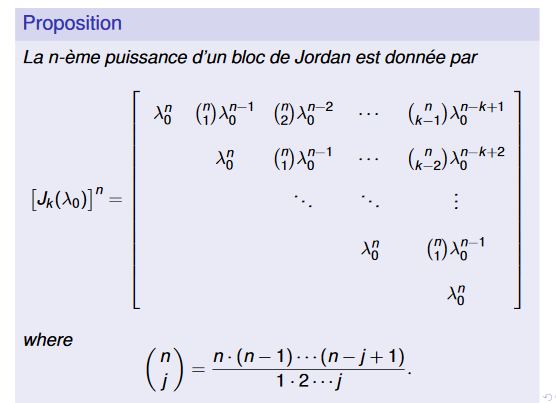
\includegraphics[width=.7\linewidth]{puissance_jordan.png}
\end{center}
\subsubsection{Solution générale}
\begin{center}
    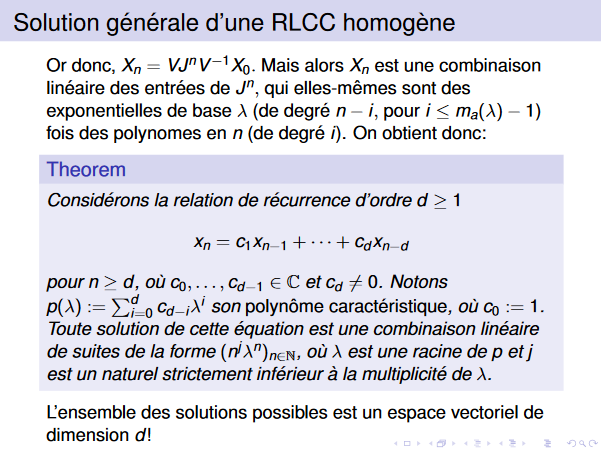
\includegraphics[width=.7\linewidth]{solution.png}
\end{center}
\subsubsection{Cas de l'équation non homogène}
L'ensemble des solutions est donné par la combili des solutions de l'équation homogène et une solution particulière de l'équation non homogène.
\subsection{EDO}
\begin{framed}
    Il existe au plus une solution au problème de Cauchy.
\end{framed}
\begin{framed}
    Si la fonction f est une combinaison linéaire de polynômes et/ou d'exponentielles, alors la solution existe et est unique.
\end{framed}
\begin{center}
    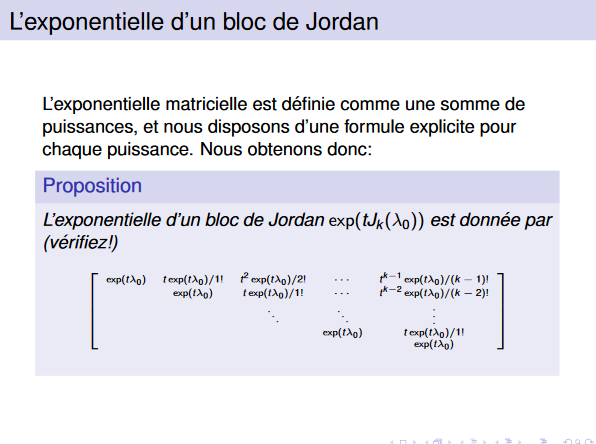
\includegraphics[width=.7\linewidth]{expo.png}
\end{center}
\begin{center}
    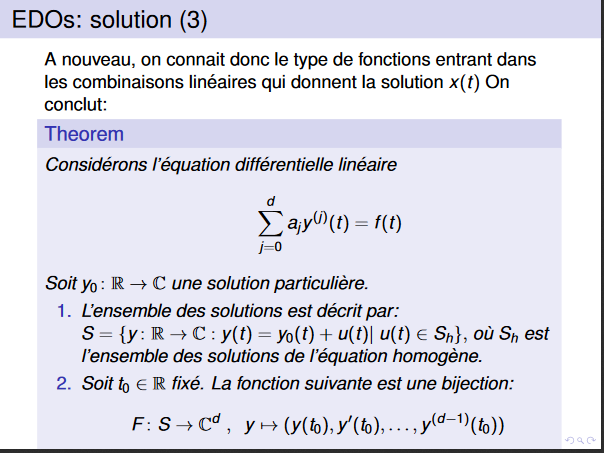
\includegraphics[width=.7\linewidth]{edo.png}
\end{center}






















\end{document}
